\documentclass[10pt, a4paper]{beamer}

\usepackage{graphicx}

\usetheme{Berkeley}
\usecolortheme{sidebartab}

\begin{document}
	\setbeamertemplate{sidebar left}{}
	\title{Progress Presentation-I}
	\subtitle{e-Yantra Summer Internship-2018
	\vspace{0.1cm}
	\\ NLP-Smart Assistant for eYantra IOT
	\\\&
	\\IFTTT for IOT}
	\author{
	Team:
	\\Onkar J. Sathe
	\\Rohit G. Rathi
	\vspace{0.2cm}
	\\Mentors:
	\\Omkar Manjrekar
	\\Vikrant Fernandes
	\\Deepa Avudiappan}
	\institute{IIT Bombay}
	\date{\today}
	%\addtobeamertemplate{sidebar left}{}{\includegraphics[scale = 0.3]{logowithtext.png}}
	\frame{\titlepage}

\setbeamertemplate{sidebar left}[sidebar theme]
\section{Overview of Project}
\begin{frame}{Overview of Project}
	NLP-Smart Assistant for eYantra IOT
	\begin{itemize}
		\item Objective
		\begin{enumerate}	
			\item Building a NLP based assistant to access eYantra IOT platform  through text and voice control over the Web portal and through Google Assistant!
		\end{enumerate}
		\item Deliverables 
		\begin{enumerate}
			\item The assistant should at least be able to perform all the frequent queries that take place on IoT platform.
			\item User should see device data in the chat interface itself.
			\item A web chatbot interface to be integrated with IoT Platform
		\end{enumerate}
	\end{itemize}
\end{frame}

\section{Overview of Task}
\begin{frame}{Overview of Task}
   % Please add the following required packages to your document preamble:
% \usepackage{graphicx}
\begin{table}[]
\resizebox{\textwidth}{!}{%
\begin{tabular}{|c|c|c|}
\hline
Task.no & Task & Deadline \\ \hline
1 & Understanding e-Yantra IoT Platform and its APIs & 2 days \\ \hline
2 & \begin{tabular}[c]{@{}c@{}}
Getting familiar with Dialogflow and \\ required programming languages\end{tabular} & 3 days \\ \hline
3 & \begin{tabular}[c]{@{}c@{}}Gathering phrases to train the agent.
\end{tabular} & 3 days \\ \hline
4 & \begin{tabular}[c]{@{}c@{}}Adding entities and intents 
\end{tabular} & 3 days \\ \hline
5 & \begin{tabular}[c]{@{}c@{}}
Take actions on the output of phrases\\ returned by API properly and ask for\\ missing information if any
\end{tabular} & 2 day \\ \hline
6 & \begin{tabular}[c]{@{}c@{}}
Testing this and the speech interface\\ and retraing on more examples if required.\end{tabular} & 3 days \\ \hline
\end{tabular}%
}
\end{table}
\end{frame}

\begin{frame}{}

% Please add the following required packages to your document preamble:
% \usepackage{graphicx}
\begin{table}[]
\resizebox{\textwidth}{!}{%
\begin{tabular}{|c|c|c|}
\hline
Task.no & Task & Deadline \\ \hline
7 & \begin{tabular}[c]{@{}c@{}}
Develop a proper web interface to \\
be integrable with IoT platform \\ designing throughout the website.\end{tabular} & 2 days \\ \hline
8 & \begin{tabular}[c]{@{}c@{}}
Integration with E-Yantra platform \\
and a demo application \\ \end{tabular} & 1 day \\ \hline
9 & \begin{tabular}[c]{@{}c@{}}
Learning VueJs and component designing \end{tabular} & 4 day \\ \hline
10 & \begin{tabular}[c]{@{}c@{}}
Designing algorithm for converting UI bloks\\ to lambda code with loose coupling
\end{tabular} & 4 days \\ \hline
11 & \begin{tabular}[c]{@{}c@{}}
Testing and improving efficiency
\end{tabular} & 1 days \\ \hline
12 & \begin{tabular}[c]{@{}c@{}}
Documentation
\end{tabular} & 2 days \\ \hline
\end{tabular}%
}
\end{table}
\end{frame}

\section{Tasks Accomplished}
\begin{frame}{What we have done so far...}
	\begin{itemize}
		\item Understanding eYantra IoT Platform and its APIs
		\newline
		\item Learning about DialogFlow \& RasaNLU and how a virtual assistant works behind the scenes
		\newline\\\vspace{0.5cm}
		\hspace{1cm}
		
\includegraphics[totalheight=.8cm]{dialogflow.png}\hspace{1cm}
		
\includegraphics[totalheight=.7cm]{rasa.png}
		\newline
		\item Understanding the working of AWS-IoT and connecting ESP8266-DHT sensor to it for testing of the assistant
	\end{itemize}
\end{frame}

\begin{frame}{What we have done so far...}
	\begin{itemize}
		\item Teaching the assistant to talk and listen with Intents
		\item Webhook in JavaScript for providing data \& rich UI responses
		\newline\\\vspace{0.3cm}				
	\end{itemize}
	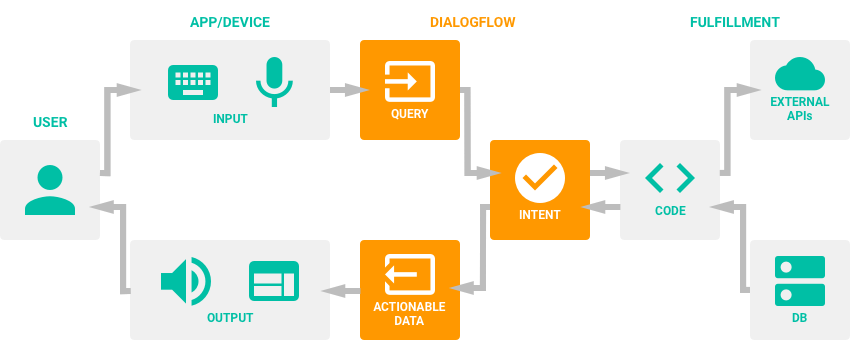
\includegraphics[totalheight=4cm]{architecture.png}
	\vspace{0.3cm}
	\\\centerline{Flow of the IoT Assistant}
\end{frame}

\begin{frame}{What we have done so far...}
	\begin{minipage}[b]{0.55\textwidth}
		\raggedright
		\begin{itemize}
			\item Integrating the IoT assistant with Google Assistant
			\newline\\\vspace{0.2cm}
			\item Secure user authentication based on OAuth2 token system
			\newline\\\vspace{0.2cm}
			\item Authenticated user can access and control devcies \& sensors on IoT platform anytime, from anywhere around the world through internet
		\end{itemize}
		\vspace{0.3cm}
	\end{minipage}%
	\begin{minipage}[b]{0.45\textwidth}
		\centering
		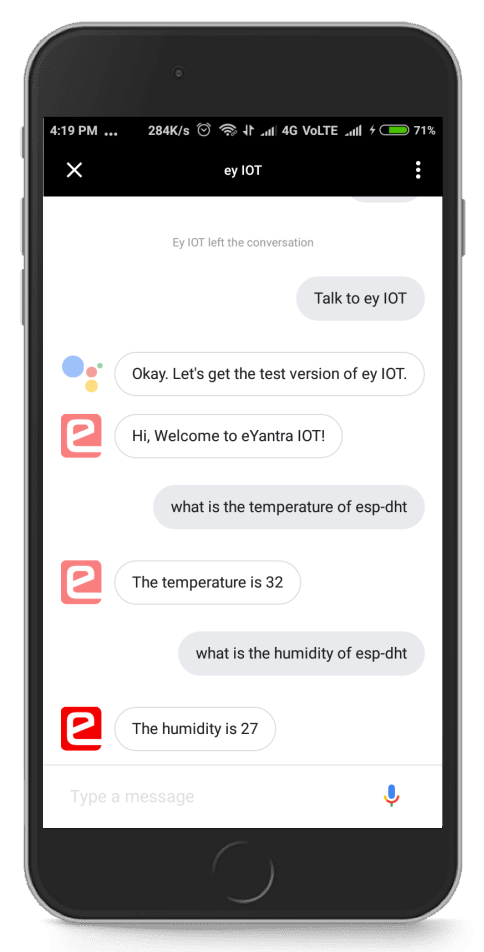
\includegraphics[totalheight=6cm]{assistant.png}
	\end{minipage}%
\end{frame}

\section{Challenges Faced}
\begin{frame}{Challenges faced and How we solved them...}
	\begin{itemize}
		\item Implementing OAuth2 Token based authentication between assistant and IoT Platform
		\newline\\
		\item Teaching the assistant to understand IoT words \& phrases like Sensor names, Units, Things and properties like temperature, humidity, etc
	\end{itemize}
\end{frame}

\section{Future Plans}
\begin{frame}{Future Plans}
	\begin{itemize}
		\item Integrating the assitant in IoT platform's website with chatbot UI
		\newline\\
		\item Making the assistant dynamic enough to handle variety of devices \& sensors with their properties
		\newline\\
		\item Assistant will be able to handle other complex commands on IoT platform like Crons from natural language and generating Rules.
	\end{itemize}
\end{frame}


\section{Thank You}
\begin{frame}{Thank You}
	\centering THANK YOU !!!
\end{frame}
\end{document}
